% \newpage\setcounter{dang}{0}
\section{CÁC KHÁI NIỆM MỞ ĐẦU}

\subsection{Tóm tắt lý thuyết}
\begin{tomtat}
	\subsubsection{Khái niệm vectơ}
	\immini{\begin{itemize}
			\item \textbf{Vectơ} là một đoạn thẳng có hướng, nghĩa là, trong hai điểm mút của đoạn thẳng, đã chỉ rõ điểm đầu, điểm cuối.
			\item \textbf{Độ dài của vectơ} là khoảng cách giữa hai điểm đầu và điểm cuối của vectơ đó.
	\end{itemize}}{\begin{tikzpicture}[scale=1, font=\footnotesize,line join=round, line cap=round, >=stealth]
			\fill (0,0) circle (1pt) node [above]{$A$} (4,0)circle (1pt) node [above]{$B$};
			\draw [->] (0,0)--(4,0);
	\end{tikzpicture}}

	\subsubsection{Hai vectơ cùng phương, cùng hướng, bằng nhau}
	\begin{center}
		\begin{tikzpicture}[scale=.8, font=\footnotesize,line join=round, line cap=round, >=stealth]
			\fill (0,0) circle (1pt) node [left]{$A$} (4,0)circle (1pt) node [right]{$B$};
			\draw [->] (0,0)--(4,0);
			\fill (-1,-1) circle (1pt) node [left]{$C$} (5,-1)circle (1pt) node [right]{$D$};
			\draw [->] (-1,-1)--(5,-1);
			\fill (7,-1) circle (1pt) node [left]{$C$} (13,-1)circle (1pt) node [right]{$D$};
			\draw [->] (7,-1)--(13,-1);
			\fill (8,-1) circle (1pt) node [above]{$B$} (12,-1)circle (1pt) node [above]{$A$};
			\draw [<-,thick] (8,-1)--(12,-1);
		\end{tikzpicture}
	\end{center}
	\begin{itemize}
		\item Đường thẳng đi qua điểm đầu và điểm cuối của một vectơ được gọi là \textbf{giá} của vectơ đó.
		\item Hai vectơ được gọi là \textbf{cùng phương} nếu chúng có giá song song hoặc trùng nhau.
		\item Đối với hai vectơ cùng phương thì chúng \textbf{cùng hướng} hoặc \textbf{ngược hướng}.
		\item Hai vectơ $\vec{a}$ và $\vec{b}$ được gọi là \textbf{bằng nhau}, kí hiệu $\vec{a}=\vec{b}$, nếu chúng có cùng độ dài và cùng hướng.
	\end{itemize}
	\begin{vd}%[0H1B1-1]
		Cho hình bình hành $ABCD$. Hãy chỉ ra các vectơ (khác $\overrightarrow{0}$) có điểm đầu và điểm cuối là một trong bốn đỉnh của hình bình hành $ABCD$. Trong số các vectơ trên, hãy chỉ ra
		\begin{enumerate}
			\item Các vectơ cùng phương.
			\item Các cặp vectơ cùng phương nhưng ngược hướng.
			\item Các cặp vectơ bằng nhau.
		\end{enumerate}
		\loigiai
		{
			\immini
			{
				Các vectơ (khác $\overrightarrow{0}$) có điểm đầu và điểm cuối là một trong bốn đỉnh của hình bình hành $ABCD$ là $\overrightarrow{AB}$, $\overrightarrow{BA}$, $\overrightarrow{AC}$, $\overrightarrow{CA}$, $\overrightarrow{AD}$, $\overrightarrow{DA}$, $\overrightarrow{BC}$, $\overrightarrow{CB}$, $\overrightarrow{BD}$, $\overrightarrow{DB}$, $\overrightarrow{CD}$, $\overrightarrow{DC}$.
			}
			{
				\begin{tikzpicture}
					\tkzDefPoints{0/0/A, 3/0/B, 4/1/C}
					\tkzDefPointBy[translation=from B to A](C)\tkzGetPoint{D}
					\tkzDrawPoints[fill=black](A,B,D,C)
					\tkzDrawPolygon(A,B,C,D)
					\tkzLabelPoints[left](A,D)
					\tkzLabelPoints[right](B,C)
				\end{tikzpicture}
			}
			\noindent
			\begin{enumerate}
				\item Các vectơ cùng phương với nhau là
				\begin{itemize}
					\item $\overrightarrow{AB}$, $\overrightarrow{BA}$, $\overrightarrow{CD}$, $\overrightarrow{DC}$.
					\item $\overrightarrow{AD}$, $\overrightarrow{DA}$, $\overrightarrow{BC}$, $\overrightarrow{CB}$.
					\item $\overrightarrow{AC}$ và $\overrightarrow{CA}$.
					\item $\overrightarrow{BD}$ và $\overrightarrow{DB}$.
				\end{itemize}
				\item Các cặp vectơ cùng phương nhưng ngược hướng là $\overrightarrow{AB}$ và $\overrightarrow{BA}$; $\overrightarrow{BC}$ và $\overrightarrow{CB}$; $\overrightarrow{CD}$ và $\overrightarrow{DC}$; $\overrightarrow{DA}$ và $\overrightarrow{AD}$; $\overrightarrow{AC}$ và $\overrightarrow{CA}$; $\overrightarrow{BD}$ và $\overrightarrow{DB}$; $\overrightarrow{AB}$ và $\overrightarrow{CD}$; $\overrightarrow{BA}$ và $\overrightarrow{DC}$; $\overrightarrow{AD}$ và $\overrightarrow{CB}$; $\overrightarrow{DA}$ và $\overrightarrow{BC}$.
				\item Các cặp vectơ bằng nhau là $\overrightarrow{AB}$ và $\overrightarrow{DC}$; $\overrightarrow{BA}$ và $\overrightarrow{CD}$; $\overrightarrow{AD}$ và $\overrightarrow{BC}$; $\overrightarrow{DA}$ và $\overrightarrow{CB}$.
			\end{enumerate}
		}
	\end{vd}
	\begin{vd}%[0H1B1-2]
		Cho hình bình hành $ABCD$. Gọi $E, F, M$ và $N$ lần lượt là trung điểm của cạnh $AB, BC, CD$ và $DA$.
		\begin{enumerate}
			\item 	Chứng tỏ rằng 3 vectơ $\overrightarrow{EF},\overrightarrow{AC},\overrightarrow{MN}$ cùng phương;
			\item Chứng tỏ rằng $\overrightarrow{EF}=\overrightarrow{NM}$. Suy ra tứ giác $EFMN$ là hình bình hành.
		\end{enumerate}
		\loigiai{
			\immini{\begin{enumerate}
					\item 	Dựa vào tính chất đường trung bình, ta suy ra được $EF\parallel AC\parallel MN\Rightarrow\overrightarrow{EF},\overrightarrow{AC},\overrightarrow{MN}$ cùng phương;
					\item Dựa vào tính chất đường trung bình, ta suy ra được $EF=MN=\dfrac{1}{2}AC$ kết hợp với câu a) $\Rightarrow\overrightarrow{EF}=\overrightarrow{NM}$. Suy ra tứ giác $EFMN$ là hình bình hành.
			\end{enumerate}}{
				\begin{tikzpicture}[>=stealth,line cap=round,line join=round, scale=.6]
					%Định nghĩa các điểm
					\tkzDefPoints{0/0/B, 2/5/A, 7/0/C}
					\coordinate(D) at ($(A)+(C)$);
					%\coordinate(M) at ($(A)-(B)+(A)$);
					%\coordinate(P) at ($(A)-(D)+(A)$);
					%\coordinate(N) at ($(A)-(B)+(P)$);
					%Gán tên các điểm
					\tkzDefMidPoint(A,B)\tkzGetPoint{E}
					\tkzDefMidPoint(B,C)\tkzGetPoint{F}
					\tkzDefMidPoint(C,D)\tkzGetPoint{M}
					\tkzDefMidPoint(D,A)\tkzGetPoint{N}
					\tkzLabelPoints[below](B,C,F)
					\tkzLabelPoints[left](E)
					\tkzLabelPoints[right](M)
					\tkzLabelPoints[above](A,D,N)
					%Nối các đường
					\tkzDrawPolygon(A,B,C,D)
					\tkzDrawPolygon(E,F,M,N)
					\tkzDrawSegments(A,C)
			\end{tikzpicture}}
		}
	\end{vd}
\end{tomtat}


\subsection{Các dạng toán thường gặp}
\begin{dang}{Xác định một vectơ}
	\begin{itemize}
		\item Vectơ là một đoạn thẳng có hướng. Vectơ có điểm đầu $A$ và điểm cuối $B$ được kí hiệu là $\overrightarrow{AB}$.
	\end{itemize}
\end{dang}
\begin{vd}%[0H4Y7-1]
	Cho hai điểm phân biệt $A,~B$. Tìm số vectơ được tạo thành từ hai điểm này?
	\loigiai{

	Vectơ là đoạn thẳng được định hướng. Như vậy từ hai điểm $A,B$ ta được hai vectơ là $\overrightarrow{AB}$ và $\overrightarrow{BA}$.
}
\end{vd}
\begin{vd}%[0H4Y7-1]
	Cho tam giác $ABC$. Viết tất cả các vectơ mà điểm đầu và điểm cuối là $A$, $B$ hoặc $C$.
	\loigiai{
		Ta có $\overrightarrow{AB}$, $\overrightarrow{BA}$, $\overrightarrow{AC}$, $\overrightarrow{CA}$, $\overrightarrow{CB}$, $\overrightarrow{BC}$.
	}
	\end{vd}


\begin{dang}{Sự cùng phương và hướng của hai vectơ}
	\begin{itemize}
		\item Hai vectơ được gọi là cùng phương nếu chúng có giá song song hoặc trùng nhau.
		\item Đối với hai vectơ cùng phương thì chúng cùng hướng hoặc ngược hướng.
	\end{itemize}
\end{dang}
\begin{vd}%[0H4B7-2]
	\immini{Cho hình thang cân $ABCD$ với hai đáy $AB$, $CD$, $AB<CD$. Hãy chỉ ra mối quan hệ về độ dài, phương, hướng giữa các cặp vectơ $\overrightarrow{AD}$ và $\overrightarrow{BC}$, $\overrightarrow{AB}$ và $\overrightarrow{CD}$, $\overrightarrow{AC}$ và $\overrightarrow{BD}$. Có cặp vectơ nào trong các cặp vectơ trên bằng nhau hay không?  }
	{\begin{tikzpicture}[scale=0.7,>=stealth, font=\footnotesize, line join=round, line cap=round]
			\coordinate (D) at (0,0);
			\coordinate (C) at (6,0);
			\coordinate (A) at (2,3);
			\coordinate (B) at (4,3);
			\draw (A)--(B)--(C)--(D)--cycle;
			\draw (A)--(C) (B)--(D);
			\foreach 	\x/ \goc in {A/180,D/180,C/0,B/0}
			\fill (\x) circle (1pt)	($(\x)+(\goc:3mm)$) node {$\x$};
	\end{tikzpicture}}
	\loigiai{
		\begin{itemize}
			\item $\left|\overrightarrow{AD}\right|=\left|\overrightarrow{BC}\right|$, $\left|\overrightarrow{AC}\right|=\left|\overrightarrow{BD}\right|$, $\left|\overrightarrow{AB}\right|<\left|\overrightarrow{DC}\right|$.
			\item $\overrightarrow{AD}$ và $\overrightarrow{BC}$,  $\overrightarrow{AC}$ và $\overrightarrow{BD}$ không cùng phương.
			\item $\overrightarrow{AB}$ và $\overrightarrow{CD}$ ngược hướng.
			\item Không có cặp vectơ nào trong các cặp vectơ trên bằng nhau.
		\end{itemize}
		}
\end{vd}

\begin{vd}%[0H4B7-2]
	Trong hình 1.4, hãy chỉ ra các vectơ cùng phương, cùng hướng, ngược hướng và các vectơ bằng nhau.
	\begin{center}
		\begin{tikzpicture}[>=stealth]
			\draw[thin,step=1cm] (-7,-2)grid(8,3);
			\draw[->,very thick] (-7,0)--(-5,2);\draw ($(-7,0)!.5!(-5,2)$) node[left]{$\vec{a}$};
			\draw[->,very thick] (-7,-2)--(-3,2);\draw ($(-7,-2)!.5!(-3,2)$) node[above left]{$\vec{b}$};
			\draw[->,very thick] (-2,2)--(1,2);\draw ($(-2,2)!.5!(1,2)$) node[above]{$\vec{x}$};
			\draw[->,very thick] (0,1)--(3,1);\draw ($(0,1)!.5!(3,1)$) node[above]{$\vec{y}$};
			\draw[->,very thick] (4,0)--(8,0);\draw ($(4,0)!.5!(8,0)$) node[below right]{$\vec{z}$};
			\draw[->,very thick] (-2,0)--(1,-1);\draw ($(-2,0)!.5!(1,-1)$) node[below]{$\vec{u}$};
			\draw[->,very thick] (4,-1)--(1,0);\draw ($(4,-1)!.5!(1,0)$) node[above]{$\vec{v}$};
			\draw[->,very thick] (7,2)--(2,2);\draw ($(7,2)!.5!(2,2)$) node[above]{$\vec{w}$};
			\fill (-7,0)circle(1.5pt) (-7,-2)circle(1.5pt) (-2,2)circle(1.5pt) (0,1)circle(1.5pt) (4,0)circle(1.5pt) (-2,0)circle(1.5pt) (4,-1)circle(1.5pt) (7,2)circle(1.5pt);
			\draw (0.5,-2.5) node{Hình 1.4};
		\end{tikzpicture}
	\end{center}
	\loigiai{\begin{itemize}
			\item Các vectơ cùng phương: $\overrightarrow{a}$ và $\overrightarrow{b}$; $\overrightarrow{u}$ và $\overrightarrow{v}$; $\overrightarrow{x}$, $\overrightarrow{y}$, $\overrightarrow{z}$ và $\overrightarrow{w}$.\\
		\item  Các vectơ cùng hướng: $\overrightarrow{a}$ và $\overrightarrow{b}$; $\overrightarrow{x}$, $\overrightarrow{y}$ và $\overrightarrow{z}$.\\
		\item Các vectơ ngược hướng: $\overrightarrow{u}$ và $\overrightarrow{v}$; $\overrightarrow{w}$ và $\overrightarrow{x}$; $\overrightarrow{w}$ và $\overrightarrow{y}$; $\overrightarrow{w}$ và $\overrightarrow{z}$.\\
		\item  Các vectơ bằng nhau: $\overrightarrow{x}=\overrightarrow{y}$.
			\end{itemize}
	}
\end{vd}

\begin{dang}{Hai vectơ bằng nhau, độ dài của vectơ}
	\begin{itemize}
		\item $\left|\overrightarrow{AB}\right|=AB$.
		\item Hai vectơ được gọi là bằng nhau nếu chúng có cùng độ dài và cùng hướng.
	\end{itemize}
\end{dang}

\begin{vd}
	\immini{Cho tam giác đều $ABC$ với cạnh có độ dài bằng $a$. Hãy chỉ ra các vectơ có độ dài bằng $a$ và có điểm đầu, điểm cuối là các đỉnh của tam giác $ABC$.
	}
	{\begin{tikzpicture}[scale=0.7, font=\footnotesize, line join=round, line cap=round, >=stealth]
			\def\bc{4} % cạnh BC
			\def\ba{4} % cạnh BA
			\def\h{4} % đường cao
			\def\gocB{60} % góc B của đáy
			\coordinate[label=below left:$B$] (B) at (0,0);
			\coordinate[label=above:$A$] (A) at (\gocB:\ba);
			\coordinate[label=below:$C$] (C) at (\bc,0);
			\draw (A)--(B)--(C)--(A);
			\foreach \diem in {A,B,C}	\fill (\diem)circle(1.5pt);
	\end{tikzpicture}}
	\loigiai{
		$\left|\overrightarrow{AB}\right|=\left|\overrightarrow{BA}\right|=\left|\overrightarrow{AC}\right|=\left|\overrightarrow{CA}\right|=\left|\overrightarrow{BC}\right|=\left|\overrightarrow{CB}\right|=a$.
	}
\end{vd}

\begin{vd}
	\immini{Cho hình bình hành $ABCD$ như hình vẽ.}
	{\begin{tikzpicture}[scale=0.8,>=stealth, font=\footnotesize, line join=round, line cap=round]
			\def\l{3}
			\def\n{5}
			\path 	(0:0) coordinate (D)
			++(0:\n) coordinate (C)
			++(50:\l) coordinate (B)
			($(B)+(D)-(C)$) coordinate (At)
			($(B)+(180:\n)$) coordinate (A);
			\draw (A)--(B)--(C)--(D)--cycle;
			\foreach 	\x/ \goc in {A/180,D/180,C/0,B/0}
			\fill (\x) circle (1pt)	($(\x)+(\goc:3mm)$) node {$\x$};
	\end{tikzpicture}}
	\begin{multicols}{2}
		\begin{enumerate}
			\item Vectơ nào bằng vectơ $\overrightarrow{AB}$?
			\item Vectơ nào bằng vectơ $\overrightarrow{AD}$?
		\end{enumerate}
	\end{multicols}
	\loigiai{\begin{multicols}{2}
			\begin{enumerate}
				\item $\overrightarrow{AB}=\overrightarrow{DC}$.
				\item $\overrightarrow{AD}=\overrightarrow{BC}$.
			\end{enumerate}
	\end{multicols}}
\end{vd}

\begin{vd}%[0H1B1-1]
	Cho hình vuông $ABCD$ cạnh $a$. Gọi $M$ là trung điểm của $AB$, $N$ là điểm đối xứng với $C$ qua $D$. Hãy tính độ dài của vectơ $\vec{MD}$ và $\vec{MN}$.
	\loigiai{
		\immini{
			Áp dụng định lý Pythagoras trong tam giác vuông $MAD$ ta có
			\[
			DM^2=AM^2+AD^2=\left (\dfrac{a}{2} \right )^2+a^2=\dfrac{5a^2}{4}\Rightarrow DM=\dfrac{a\sqrt{5}}{2}
			\]
			Suy ra $\left |\vec{MD}\right |=MD=\dfrac{a\sqrt{5}}{2}$.\\
			Qua $N$ kẻ đường thẳng song song với $AD$ cắt $AB$ tại $P$.\\
			Khi đó tứ giác $ADNP$ là hình vuông và $PM=PA+AM=a+\dfrac{a}{2}=\dfrac{3a}{2}$.\\
			Áp dụng định lý Pythagoras trong tam giác vuông $NPM$ ta có
			\[
			MN^2=NP^2+PM^2=a^2+\left (\dfrac{3a}{2} \right )^2=\dfrac{13a^2}{4}\Rightarrow MN=\dfrac{a\sqrt{13}}{2}
			\]
			Suy ra $\left |\vec{MN}\right |=MN=\dfrac{a\sqrt{13}}{2}$.
		}{
			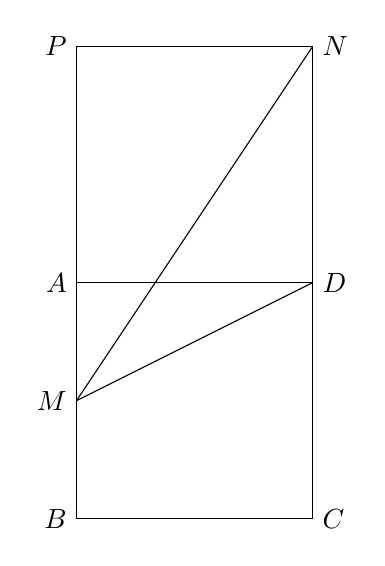
\begin{tikzpicture}[scale=3]
				\draw(1.,1.)-- (1.,0.);
				\draw(1.,0.)-- (2.,0.);
				\draw(2.,0.)-- (2.,1.);
				\draw(2.,1.)-- (1.,1.);
				\draw(2.,1.)-- (2.,2.);
				\draw(2.,2.)-- (1.,2.);
				\draw(1.,2.)-- (1.,1.);
				\draw(1,0.5)-- (2.,1.);
				\draw(1,0.5)-- (2.,2.);
				\draw(1,1) node [left]{$A$};
				\draw(1,0) node [left]{$B$};
				\draw(2,0) node [right]{$C$};
				\draw(2,1) node [right]{$D$};
				\draw(2,2) node [right]{$N$};
				\draw(1,2) node [left]{$P$};
				\draw(1,0.5) node  [left]{$M$};
			\end{tikzpicture}
		}

	}
\end{vd}


\subsection{Bài tập}
\subsubsection{Bài tập tự luận}
\begin{bt}%[Trong Nguyen]%[0H1Y1-2]
	Cho ba vec-tơ $ \vec{a} $, $ \vec{b} $, $ \vec{c} $ đều khác $ \vec{0} $.
	Những khẳng định nào sau đây là đúng?
		\begin{enumerate}
		\item  $ \vec{a} $, $ \vec{b} $, $ \vec{c} $ đều cùng hướng với $
		\vec{0} $.
		\item Nếu $ \vec{b} $ không cùng hướng với $ \vec{a} $ thì $ \vec{b} $
		ngược hướng với $ \vec{a} $.
		\item Nếu $ \vec{a} $ và $ \vec{b} $ đều cùng phương với $ \vec{c} $
		thì $ \vec{a} $ và $ \vec{b} $  cùng phương.
		\item  Nếu $ \vec{a} $ và $ \vec{b} $ đều cùng hướng với $ \vec{c} $
		thì $ \vec{a} $ và $ \vec{b} $  cùng hướng.
	\end{enumerate}
\loigiai{
	\begin{enumerate}
		\item Khẳng định đúng.
		\item Khẳng định sai.
		\item Khẳng định đúng.
		\item Khẳng định đúng.
	\end{enumerate}
}
\end{bt}
\begin{bt}%[Trong Nguyen]%[0H1Y1-2]
	\immini
	{
		Trong hình $ 4.12 $, hãy chỉ ra các vectơ cùng phương, các cặp vectơ
		ngược hướng và các cặp vectơ bằng nhau.
	}
	{
		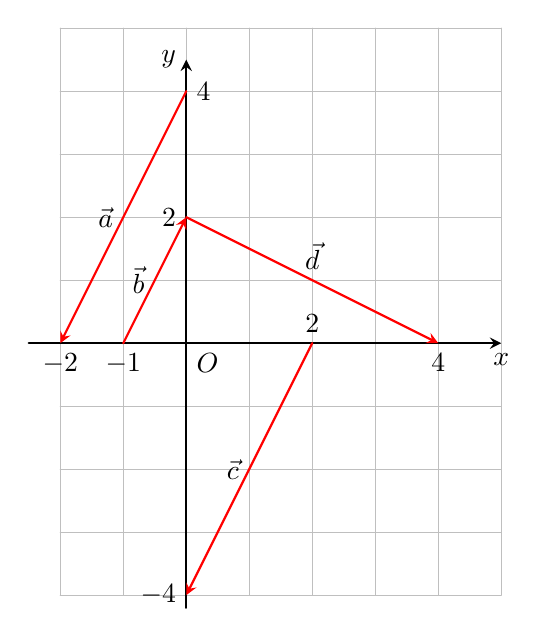
\begin{tikzpicture}[line join=round, line
		cap=round,>=stealth,thick,scale = 0.8]
\draw[gray!50,thin,opacity=1]
(-2,-4) grid (5,5);
\def \xmin{-2.5}
\def \xmax{5}
\def \ymin{-4.2}
\def \ymax{4.5}
\draw[->] (\xmin,0)--(\xmax,0) node[below] {$x$};
\draw[->] (0,\ymin)--(0,\ymax) node[left] {$y$};
\draw (0,0) node [below right] {$O$};
\draw[->,red] (0,4) node[right,black]{$ 4 $}--(-2,0)node[below,black]{$ -2 $}
node[midway,left,black]{$ \vec{a} $};
\draw[->,red] (-1,0)node[below,black]{$ -1 $}--(0,2)node[left,black]{$ 2 $}
node[midway, left,black]{$ \vec{b} $};
\draw[->,red] (2,0)node[above,black]{$ 2 $}-- (0,-4)node[left,black]{$ -4 $}
node[midway, left,black]{$ \vec{c} $};
\draw[->,red] (0,2)--(4,0)node[below,black]{$ 4
$}  node[midway, above,black]{$ \vec{d} $};
\end{tikzpicture}
	}
\loigiai{
	\begin{itemize}
		\item Các vectơ cùng phương: $ \vec{a} $, $ \vec{b} $, $ \vec{c} $.
		\item Các cặp vectơ ngược hướng: $ \vec{a} $ và $ \vec{b} $, $ \vec{b}
		$ và $ \vec{c} $.
		\item Các cặp vectơ bằng nhau: $ \vec{a} $ và $ \vec{c} $.
	\end{itemize}
}
\end{bt}

\begin{bt}%[Trong Nguyen]%[0H1B1-2]
	Chứng minh rằng tứ giác $ ABCD $ là hình bình  khi và chỉ khi $ \vec{BC} =
	\vec{AD} $.
	\loigiai{
		\immini
		{
		\begin{itemize}
			\item Giả sử $ ABCD $ là hình bình hành. \\
			Khi đó $ BC \parallel AD \Rightarrow \vec{BC} $ cùng phương
			$ \vec{AD} $.\\
			Lại có $ BC=AD $ nên độ lớn của $ 2 $ vec tơ $
			\vec{BC} $ và $ \vec{AD} $ bằng nhau. Vậy  $ \vec{BC} =
			\vec{AD} $.
			\item Giả sử $ \vec{BC} = \vec{AD} $. \\
			Khi đó $ BC \parallel AD $ và $ BC=AD $ nên tứ giác $ ABCD $ là
			hình bình hành.
 		\end{itemize}
	}
{
	\begin{tikzpicture}[>=stealth,scale=1, line join = round, line cap
	= round]
	\coordinate (A) at (0,0);
	\coordinate (B) at (3,0);
	\coordinate (C) at (4,2);
	\coordinate (D) at ($(A)+(C)-(B)$);
	\draw (A) node[left] {$ A $}--(B)node[right] {$ B $}
	(C)node[right] {$ C $}--(D)node[left] {$ D $};
	\draw[->] (B)--(C);
	\draw[->] (A)--(D);
	\end{tikzpicture}
}
	}

\end{bt}

\begin{bt}%[Trong Nguyen]%[0H1K1-2]
	Trên mặt phẳng tọa độ $ Oxy $, hãy vẽ các vectơ $ \vec{OA} $, $ \vec{MN} $
	với $ A(1;2) $, $ M(0;-1) $, $ N(3;5) $.
	\begin{enumerate}
		\item Hãy chỉ ra mối liên hệ giữa các vectơ trên.
		\item Một vật thể khởi hành từ $ M $ và chuyển động thẳng đều với vận
		tốc (tính theo giờ) được biểu diễn bởi vectơ $ \vec{v}=\vec{OA} $. Hỏi
		vật thể đó qua $ N $ hay không? nếu có thì sau bao lâu vật sẽ tới $ N $?
	\end{enumerate}
	\loigiai{
		\immini
		{
			\begin{enumerate}
				\item Gọi $ I(0,2) $, $ K(0,5) $.\\
				Ta có $ \dfrac{AI}{NK}=\dfrac{OI}{MK}=\dfrac{1}{3} \Rightarrow
				\triangle AIO \backsim \triangle{NKM}$.\\
				Suy ra $ \widehat{AOI} =\widehat{NMK} \Rightarrow OA \parallel
				MN$. \\
				Vậy $ \vec{OA} $ cùng hướng với $ \vec{MN} $.
				\item Do $ \vec{OA} $ cùng hướng với $ \vec{MN} $ nên khi vật
				thể khởi hành từ $ M $ và chuyển động thẳng đều với vận tốc
				được biểu diễn bởi vec tơ $ \vec{v} = \vec{OA} $ sẽ đi qua $ N
				$.\\
				Lại có
				$\dfrac{AI}{NK}=\dfrac{OI}{MK}=\dfrac{OA}{MN}=\dfrac{1}{3}
				\Rightarrow MN=3OA $. \\
				Suy ra $\left|\vec{MN}\right|  = 3	\left|\vec{OA}\right| $.\\
				Vậy sau $ 3 $ giờ thì vật sẽ tới $ N $.
			\end{enumerate}
		}
		{
		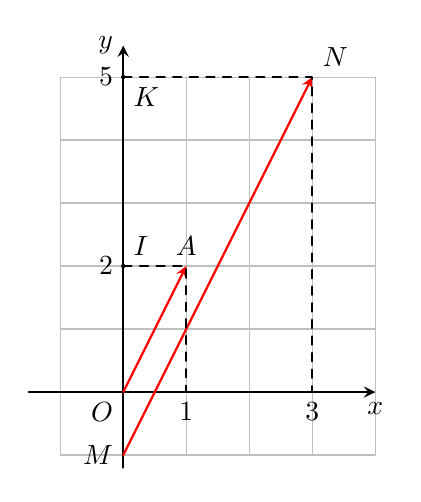
\begin{tikzpicture}[line join=round, line
		cap=round,>=stealth,thick,scale = 0.8]
		\draw[gray!50,thin,opacity=1]
		(-1,-1) grid (4,5);
		\def \xmin{-1.5}
		\def \xmax{4}
		\def \ymin{-1.2}
		\def \ymax{5.5}
		\draw[->] (\xmin,0)--(\xmax,0) node[below] {$x$};
		\draw[->] (0,\ymin)--(0,\ymax) node[left] {$y$};
		\draw (0,0) node [below left] {$O$};
		\draw[->,red] (0,0) --(1,2) node[above,black]{$ A $};
		\draw[->,red] (0,-1)node[left,black]{$ M $} --(3,5) node[above
		right,black]{$
		N $};
		\draw[dashed] (0,2) node[left]{$ 2 $}--(1,2)--(1,0)node[below]{$ 1 $};
		\draw[dashed] (0,5) node[left]{$ 5 $}--(3,5)--(3,0) node[below]{$ 3 $};
		\fill[black] (0,2) node[above right]{$ I $} circle(1pt) (0,5)
		node[below right]{$ K $} circle(1pt);
		\end{tikzpicture}
		}
	}
\end{bt}

\begin{bt}%[Trong Nguyen]%[0H1Y1-2]
	Cho $ A $, $ B $, $ C $ là ba điểm thẳng hàng, $ B $ nằm giữa $ A $ và $ C
	$. Viết các cặp vectơ cùng hướng, ngược hướng trong những vactơ sau: $
	\vec{AB} $, $ \vec{AC} $, $ \vec{BA} $, $ \vec{BC} $, $ \vec{CA} $, $
	\vec{CB} $.
	\loigiai{
		\immini
		{
			\begin{itemize}
			\item Các cặp vectơ cùng hướng gồm: $ \vec{AB} $ và $ \vec{BC} $, $
			\vec{AB} $ và $ \vec{AC} $, $ \vec{AC} $ và $ \vec{BC} $, $
			\vec{BA} $ và $ \vec{CB} $, $ \vec{BA} $ và $ \vec{CA} $, $
			\vec{CA} $ và $ \vec{CB} $.
			\item Các cặp vec tơ ngược hướng gồm: $ \vec{AB} $ và $ \vec{BA} $,
			$\vec{AB} $ và $ \vec{CB} $, $ \vec{AB} $ và $ \vec{CA} $, $
			\vec{AC} $ và $ \vec{BA} $, $\vec{AC} $ và $ \vec{CB} $, $ \vec{AC}
			$ và $ \vec{CA} $, $ \vec{BC} $ và $ \vec{BA} $,
			$\vec{BC} $ và $ \vec{CB} $, $ \vec{BC} $ và $ \vec{CA} $
		\end{itemize}
		}
		{
			\begin{tikzpicture}[>=stealth,scale=1, line join = round, line cap
			= round]
			\coordinate (A) at (0,0);
			\coordinate (C) at (4,0);
			\coordinate (B) at ($(A)!0.5!(C)$);
			\coordinate (D) at ($(A)+(C)-(B)$);
			\draw (A) node[below] {$ A $}--(B)node[below] {$ B $}--
			(C)node[below] {$ C $};
			\foreach \diem in {A,B,C}
			\draw[fill=black] (\diem) circle(1pt);
			\end{tikzpicture}
		}
	}
\end{bt}

\begin{bt}%[Trong Nguyen]%[0H1Y1-2]
	\immini
	{
	Quan sát ròng rọc hoạt động khi dùng lực để kéo một đầu của ròng rọc.
	Chuyển động của đoạn dây mô tả bằng các vectơ $ \vec{a} $, $ \vec{b} $, $
	\vec{c} $ (như hình vẽ).
	\begin{enumerate}
		\item Hãy chỉ ra các vectơ cùng phương.
		\item Trong các vectơ đó, cho biết chúng cùng hướng hay ngược hướng.
	\end{enumerate}
	}
	{
	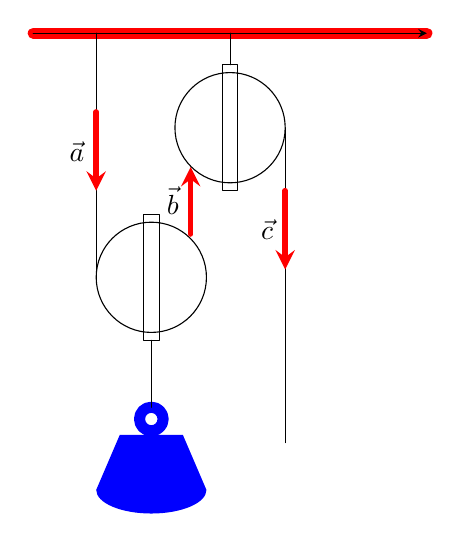
\begin{tikzpicture}[>=stealth,scale=1, line join = round, line cap
	= round]
	\def \r{.8}
	;
	\coordinate (A) at (0,0);
	\coordinate (B) at (5,0);
	\coordinate (M) at (1.5,-3.1);
	\coordinate (N) at (2.5,-1.2);
	\coordinate (K) at (1.5-\r+0.1,0);
	\coordinate (H) at (2.5+\r-0.1,-1.2);
	\tikzset{truc/.pic={	\draw(-0.1,-\r) rectangle (0.1,\r);}}
	\draw
	(M) pic[local bounding box=R1]
	{truc}
	(N) pic[local bounding box=R2]
	{truc};
	\tikzset{tron/.pic={	\draw (0,0) circle (\r-0.1);}}
	\draw
	(M) pic[local bounding box=T1]
	{tron}
	(N) pic[local bounding box=T2]
	{tron};
	\tikzset{can/.pic={
	\fill[blue](-0.4,0.4)--(-0.7,-0.3)--(-.7,-0.3) arc (-180:0:{0.7} and
	{0.3})--(0.4,0.4)--cycle;
	\draw[line width=4,blue] (0,0.6) circle(0.15);
	}}
	\draw
	(1.5,-5.5) pic[local bounding box=C]
	{can};
	\draw[line width=4,red] (A)--(B);
	\draw[->] (A)--(B);
	\draw (R1)--(C) (R2)--(2.5,0) ;
	\draw (K)--++(-90:3.1);
	\draw (H)--++(-90:4);
	\draw[->,line width=2,red] (1.5-\r+0.1,-1)--++(-90:1)
	node[midway,left,black] {$ \vec{a} $};
	\draw[->,line width=2,red]
	(2.5+\r-0.1,-2)--++(-90:1)node[midway,left,black]
	{$ \vec{c} $};
	\draw[->,line width=2,red] (2,-2.55)--++(90:.85)node[midway,left,black] {$
		\vec{b} $};
	\end{tikzpicture}
	}

	\loigiai{
		\begin{enumerate}
			\item Các vectơ cùng phương gồm: $ \vec{a} $, $ \vec{b} $, $
			\vec{c} $.
			\item Các vectơ cùng hướng gồm: $ \vec{a} $ và $ \vec{c} $. \\
			Các vectơ ngược hướng gồm: $ \vec{a} $ và $ \vec{b} $, $ \vec{b} $
			và $ \vec{c} $ .
		\end{enumerate}
	}
\end{bt}

\begin{bt}%[0H4B7-1]
	Cho bốn điểm phân biệt không thẳng hàng $A,~B,~C,~D$. Có bao nhiêu vectơ khác vectơ không có điểm đầu và điểm cuối là hai trong bốn điểm đã cho?
	\loigiai
	{Có $4$ điểm tạo thành $6$ đoạn thẳng. Mỗi đường thẳng có $2$ vectơ. Vậy có $12$ vectơ}
\end{bt}

\begin{bt}%[0H4B7-2]
	Cho tam giác $ABC$. Gọi $M$, $N$, $P$ lần lượt là trung điểm của $BC$, $CA$, $AB$.
	\begin{enumerate}
		\item Liệt kê tất cả các vectơ khác vectơ $\overrightarrow{0}$, cùng phương với $\overrightarrow{MN}$ và có điểm đầu, điểm cuối lấy trong các điểm đã cho.
		\item Liệt kê các vectơ khác vectơ $\overrightarrow{0}$, cùng hướng với $\overrightarrow{AB}$ và có điểm đầu, điểm cuối lấy trong các điểm đã cho.
	\end{enumerate}
	\loigiai{
		\begin{center}
			\begin{tikzpicture}[scale=0.8,>=stealth, font=\footnotesize, line join=round, line cap=round]
				\coordinate (A) at (3,5);
				\coordinate (B) at (0,0);
				\coordinate (C) at (10,0);
				\coordinate (M) at ($(C)!0.5!(B)$);
				\coordinate (N) at ($(A)!0.5!(C)$);
				\coordinate (P) at ($(A)!0.5!(B)$);
				%					\coordinate(A') at ($(A)+(-5,0)$);
				%				\coordinate(B') at ($(B)+(-5,0)$);
				\draw (A)--(B)--(C)--(A);
				\draw (M)--(N)--(P)--(M);
				\foreach 	\x/ \goc in {A/90,M/-90,C/0,B/-90,N/0,P/150}
				\fill (\x) circle (1pt)	($(\x)+(\goc:3mm)$) node {$\x$};
			\end{tikzpicture}
		\end{center}
		\begin{enumerate}
			\item Các vectơ khác vectơ $\overrightarrow{0}$, cùng phương với $\overrightarrow{MN}$ là $\overrightarrow{NM}, \overrightarrow{AB}, \overrightarrow{BA}, \overrightarrow{AP}, \overrightarrow{PA}, \overrightarrow{BP}, \overrightarrow{PB}$.
			\item Các vectơ khác vectơ $\overrightarrow{0}$, cùng hướng với $\overrightarrow{AB}$ là $\overrightarrow{AP}, \overrightarrow{PB}, \overrightarrow{NM}$.
		\end{enumerate}
	}
\end{bt}

\begin{bt}%[0H1B7-3]
	Cho hình thang vuông tại $A$ và $D$ có $AB=AD=a$, $\widehat{C}=45^\circ$.
	\begin{multicols}{2}
		\begin{enumerate}
			\item Tính $\left|\overrightarrow{CD}\right|$.
			\item Tính $\left|\overrightarrow{BD}\right|$.
		\end{enumerate}
	\end{multicols}
	\loigiai{\begin{center}
			\begin{tikzpicture}[scale=0.7,>=stealth, font=\footnotesize, line join=round, line cap=round]
				\coordinate (D) at (0,0);
				\coordinate[label=above left:\tiny{$45^\circ$}] (C) at (6,0);
				\coordinate (A) at (0,3);
				\coordinate (B) at (3,3);
				\coordinate (I) at ($(D)!0.5!(C)$);
				\draw (A)--(B)--(C)--(D)--cycle;
				\draw (B)--(I);
				\foreach 	\x/ \goc in {A/180,D/180,C/0,B/0,I/-60}
				\fill (\x) circle (1pt)	($(\x)+(\goc:3mm)$) node {$\x$};
				\pic[draw,angle radius=2mm]{right angle=B--A--D};
				\pic[draw,angle radius=2mm]{ angle=B--C--D};
				\pic[draw,angle radius=2mm]{right angle=I--D--A};
			\end{tikzpicture}
		\end{center}
		Gọi $I$ là trung điểm của $CD$. Khi đó $ABDI$ là hình vuông có cạnh là $a$ và tam giác $BCI$ vuông cân tại $I$.
		\begin{multicols}{2}
			\begin{enumerate}
				\item $\left|\overrightarrow{CD}\right|=CD=2a$.
				\item $\left|\overrightarrow{BD}\right|=BD=a\sqrt{2}$.
			\end{enumerate}
	\end{multicols}}
\end{bt}

\begin{bt}%[0H4B7-3]
	Cho hình vuông $ABCD$ cạnh $a$. Gọi $M$ là trung điểm của $AB$, $N$ là điểm đối xứng với $C$ qua $D$. Hãy tính độ dài của vectơ $\overrightarrow{MD}$ và $\overrightarrow{MN}$.
	\loigiai{
		\immini{
			Áp dụng định lý Pythagoras trong tam giác vuông $MAD$ ta có
			\[
			DM^2=AM^2+AD^2=\left (\dfrac{a}{2} \right )^2+a^2=\dfrac{5a^2}{4}\Rightarrow DM=\dfrac{a\sqrt{5}}{2}
			\]
			Suy ra $\left |\overrightarrow{MD}\right |=MD=\dfrac{a\sqrt{5}}{2}$.\\
			Qua $N$ kẻ đường thẳng song song với $AD$ cắt $AB$ tại $P$.\\
			Khi đó tứ giác $ADNP$ là hình vuông và $PM=PA+AM=a+\dfrac{a}{2}=\dfrac{3a}{2}$.\\
			Áp dụng định lý Pythagoras trong tam giác vuông $NPM$ ta có
			\[
			MN^2=NP^2+PM^2=a^2+\left (\dfrac{3a}{2} \right )^2=\dfrac{13a^2}{4}\Rightarrow MN=\dfrac{a\sqrt{13}}{2}
			\]
			Suy ra $\left |\overrightarrow{MN}\right |=MN=\dfrac{a\sqrt{13}}{2}$.
		}{
			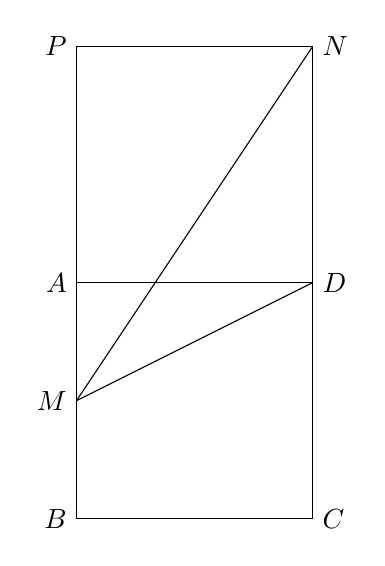
\begin{tikzpicture}[scale=3]
				\draw(1.,1.)-- (1.,0.);
				\draw(1.,0.)-- (2.,0.);
				\draw(2.,0.)-- (2.,1.);
				\draw(2.,1.)-- (1.,1.);
				\draw(2.,1.)-- (2.,2.);
				\draw(2.,2.)-- (1.,2.);
				\draw(1.,2.)-- (1.,1.);
				\draw(1,0.5)-- (2.,1.);
				\draw(1,0.5)-- (2.,2.);
				\draw(1,1) node [left]{$A$};
				\draw(1,0) node [left]{$B$};
				\draw(2,0) node [right]{$C$};
				\draw(2,1) node [right]{$D$};
				\draw(2,2) node [right]{$N$};
				\draw(1,2) node [left]{$P$};
				\draw(1,0.5) node  [left]{$M$};
			\end{tikzpicture}
		}

	}
\end{bt}

\subsubsection{Bài tập trắc nghiệm}
\Opensolutionfile{ans}
\setcounter{ex}{0}
\begin{ex}%[0H4Y7-1]
	Chọn khẳng định đúng?
	\choice
	{Vectơ là một đường thẳng có hướng}
	{Vectơ là một đoạn thẳng}
	{\True Vectơ là một đoạn thẳng có hướng }
	{Vectơ là một đoạn thẳng không phân biệt điểm đầu và điểm cuối}
	\loigiai
	{Định nghĩa vectơ}
\end{ex}
\begin{ex}%[0H4B7-1]
	Cho bốn điểm phân biệt không thẳng hàng. Hỏi có bao nhiêu vectơ được tạo thành từ bốn điểm này?
	\choice
	{$6$}
	{$8$}
	{$10$}
	{\True $12$}
	\loigiai
	{Bốn điểm phân biệt tạo thành $6$ đoạn thẳng. Suy ra có $12$ vectơ được thành lập.}
\end{ex}

\begin{ex}%[0H4B7-1]
	Cho lục giác $ABCDEF$ . Có bao nhiêu vectơ khác vectơ không có điểm đầu và điểm cuối là đỉnh của lục giác.
	\choice
	{$20$}
	{$12$}
	{\True $30$}
	{$16$}
	\loigiai{
		Hai điểm phân biệt, chẳng hạn $A,B$ ta xác định được hai vectơ khác  vectơ không là $\overrightarrow{AB},\overrightarrow{BA}$ . Một  vectơ khác  vectơ không được xác định bởi $2$ điểm phân biệt. Do đó có $30$ cách chọn $2$ điểm trong $6$ đỉnh của lục giác (có tính thứ tự các điểm) nên có thể lập được $30$ vectơ.}
\end{ex}


\begin{ex}%[0H4B7-2]
	Trong các điều kiện dưới đây. Chọn điều kiện cần và đủ để một điểm $M$ nằm giữa hai điểm phân biệt $A$ và $B$.
	\choice
	{ $\overrightarrow{AB}$ và $\overrightarrow{AM}$ ngược hướng}
	{ $\overrightarrow{MA}$ và $\overrightarrow{MB}$ cùng phương}
	{ $\overrightarrow{AB}$ và $\overrightarrow{AM}$ cùng hướng}
	{\True $\overrightarrow{MA}$ và $\overrightarrow{MB}$ ngược hướng}
	\loigiai{
		Điều kiện cần và đủ để một điểm $M$ nằm giữa hai điểm phân biệt $A$ và $B$ là $\overrightarrow{MA}$ và $\overrightarrow{MB}$ ngược hướng.
	}
\end{ex}

\begin{ex}%[0H4Y7-2]
	Phát biểu nào sau đây là sai?
	\choice
	{Hai vectơ cùng phương là hai vectơ có giá song song hoặc trùng nhau}
	{Nếu hai vectơ cùng hướng thì chúng có cùng phương}
	{Vectơ không cùng phương với mọi vectơ}
	{\True Nếu hai vectơ cùng phương thì chúng ngược hướng}
	\loigiai
	{Hai vectơ cùng phương thì chúng có thể cùng hướng hoặc ngược hướng}
\end{ex}

\begin{ex}%[0H4B7-2]
	Gọi $C$ là trung điểm của đoạn thẳng $AB$. Mệnh đề nào sau đây đúng?
	\choice
	{$\overrightarrow{CA}=\overrightarrow{CB}$}
	{\True $\overrightarrow{AB},\overrightarrow{AC}$ cùng phương}
	{$\overrightarrow{AB},\overrightarrow{CB}$ ngược hướng}
	{$|\overrightarrow{AB}|=|\overrightarrow{CB}|$}
	\loigiai
	{Vì $C$ thuộc $AB\Rightarrow A,B,C$ thẳng hàng suy ra $\overrightarrow{AB},\overrightarrow{AC}$ cùng phương}
\end{ex}


\begin{ex}%[0H4B7-2]
	Cho ba điểm $A$, $B$, $C$ phân biệt thẳng hàng. Khi nào thì hai vectơ $\overrightarrow{AB}$ và $\overrightarrow{AC}$ cùng hướng?
	\choice
	{ $A$ nằm trong đoạn $BC$}
	{ $\overrightarrow{AB}=\overrightarrow{CA}$}
	{\True $A$ nằm ngoài đoạn $BC$}
	{ $AB=AC$}
	\loigiai{
		$A$ nằm ngoài đoạn $BC$}
\end{ex}

\begin{ex}%[0H4B7-2]
	Điền từ thích hợp vào dấu (...) để được mệnh đề đúng. Hai vectơ ngược hướng thì.
	\choice
	{Bằng nhau}
	{\True Cùng phương}
	{Cùng độ dài}
	{Cùng điểm đầu}
	\loigiai{Hai vectơ ngược hướng thì cùng phương nhưng độ dài không chắc bằng nhau.}
\end{ex}

\begin{ex}%[0H4Y7-2]
	Khẳng định nào sau đây sai?
	\choice
	{Hai vectơ cùng phương với một vectơ khác vectơ không thì hai vectơ đó cùng phương}
	{ Hai vectơ cùng hướng với một vectơ khác vectơ không thì hai vectơ đó cùng hướng}
	{\True Hai vectơ ngược hướng với một vectơ khác vectơ không thì hai vectơ đó ngược hướng}
	{Hai vectơ cùng bằng một vectơ thứ ba thì hai vectơ đó bằng nhau}
	\loigiai
	{Hai vectơ ngược hướng với một vectơ khác vectơ không thì hai vectơ đó cùng hướng}
\end{ex}

\begin{ex}%[0H1B1-2]
	Cho ba điểm $A$, $B$, $C $ phân biệt thẳng hàng. Vị trí của $A$, $B$, $C$ để hai vectơ $\overrightarrow{BA}$, $\overrightarrow{BC}$ ngược hướng là
	\choice
	{\True $B$ nằm giữa $A$ và $C$}
	{$C$ nằm giữa $A$ và $B$}
	{Theo thứ tự $C$, $B$, $A$}
	{Theo thứ tự $B$, $A$, $C$}
	\loigiai
	{$\overrightarrow{BA}$, $\overrightarrow{BC}$ ngược hướng khi $B$ nằm giữa $A $ và $C$.}
\end{ex}


\begin{ex}%[0H4B7-3]
	Cho hình thoi $ABCD$. Đẳng thức nào sau đây đúng?
	\choice
	{\True $\overrightarrow{BC}=\overrightarrow{AD}$}
	{$\overrightarrow{AB}=\overrightarrow{CD}$}
	{$\overrightarrow{AC}=\overrightarrow{BD}$}
	{$\overrightarrow{DA}=\overrightarrow{BC}$}
	\loigiai
	{Theo tính chất hình bình hành}
\end{ex}

\begin{ex}%[0H4B7-3]
	Khẳng định nào sau đây đúng?
	\choice
	{\True Hai vectơ bằng nhau là hai vectơ có cùng hướng và cùng độ dài}
	{Hai vectơ bằng nhau là hai vectơ có độ dài bằng nhau}
	{Hai vectơ bằng nhau là hai vectơ có cùng giá và cùng độ dài}
	{Hai vectơ bằng nhau là hai vectơ có cùng phương và cùng độ dài}
	\loigiai
	{Theo định nghĩa hai vectơ bằng nhau}
\end{ex}

\begin{ex}%[0H4B7-3]
	Cho tam giác đều $ABC$. Khẳng định nào sau đây đúng?
	\choice
	{$\overrightarrow{AB}=\overrightarrow{AC}$}
	{$\overrightarrow{BC}=\overrightarrow{AB}$}
	{$\overrightarrow{AB}=\overrightarrow{BC}$}
	{\True $|\overrightarrow{AB}|=|\overrightarrow{AC}|$}
	\loigiai
	{Vì tam giác đều có ba cạnh bằng nhau }
\end{ex}


\begin{ex}%[0H4B7-3]
	Cho hình bình hành $ABCD$. Gọi $O$ là giao điểm của hai đường chéo . Tìm khẳng định sai
	\choice
	{$\overrightarrow{AB}=\overrightarrow{DC}$}
	{$|\overrightarrow{AB}|=|\overrightarrow{CD}|$}
	{$\overrightarrow{AO}=\overrightarrow{OC}$}
	{\True $\overrightarrow{OB}=\overrightarrow{OD}$}
	\loigiai
	{$O$ là giao điểm hai đường chéo của hình bình hành nên $O$ là trung điểm của $BD \Rightarrow \overrightarrow{OB}=-\overrightarrow{OD}$}
\end{ex}


\begin{ex}%[0H4B7-3]
	Cho hình vuông $ABCD$ tâm $O$. Khẳng định nào sau đây đúng?
	\choice
	{$\overrightarrow{AB}=\overrightarrow{CD}$}
	{$\overrightarrow{OB}=\overrightarrow{OD}$}
	{\True $|\overrightarrow{AC}|=|\overrightarrow{DB}|$}
	{$\overrightarrow{OA}=\overrightarrow{OB}$}
	\loigiai
	{Hai đường chéo hình vuông bằng nhau}
\end{ex}

\Closesolutionfile{ans}

\subsection{Luyện tập}
\subsubsection{Bài tập tự luận}

\setcounter{bt}{0}

\begin{bt}%[Trong Nguyen]%[0H1Y1-3]
	Cho hình vuông $ ABCD $ có hai đường chéo cắt nhau tại $ O $. Hãy chỉ ra
	tập hợp $ S $ gồm tất cả các vectơ khác $ \vec{0} $, có điểm đầu và điểm
	cuối thuộc tập hợp \{$ A $; $ B $; $ C $; $ D $; $ O $\}. Hãy chia tập hợp
	$ S $ thành các nhóm sao cho hai vectơ thuộc cùng một nhóm khi và chỉ khi
	chúng bằng nhau.
	\loigiai{
		\immini
		{
			Ta có
			\allowdisplaybreaks
			\begin{align}
				S =
				& \{ \vec{AB}, \vec{AC},\vec{AD}, \vec{AO}, \vec{BA},\vec{BC},
				\vec{BD},\vec{BO}, \vec{CA},\vec{CB}, \nonumber\\
				&\vec{CD}, \vec{CO}, \vec{DA}, \vec{DB}, \vec{DC},\vec{DO}, \vec{OA},
				\vec{OB}, \vec{OC}, \vec{OD} \nonumber\}
			\end{align}
		}
		{
			\begin{tikzpicture}[>=stealth,scale=1, line join = round, line cap
				= round]
				\coordinate (A) at (0,0);
				\coordinate (B) at (3,0);
				\coordinate (C) at (3,3);
				\coordinate (D) at ($(A)+(C)-(B)$);
				\draw (A) node[left] {$ A $}--(B)node[right] {$ B $}--
				(C)node[right] {$ C $}--(D)node[left] {$ D $}--cycle;
				\draw (A)--(C) (B)--(D) node[midway,above]{$ O $};
			\end{tikzpicture}
		}
		Các nhóm gồm các vectơ bằng nhau của tập $ S $ là
		\begin{itemize}
			\begin{multicols}{4}
				\item $ S_1=\left\{\vec{AB}, \vec{DC} \right\}$.
				\item $ S_2=\left\{\vec{BA}, \vec{CD} \right\}$.
				\item $ S_3=\left\{\vec{AD}, \vec{BC} \right\}$.
				\item $ S_4=\left\{\vec{DA}, \vec{CB} \right\}$.
				\item $ S_5=\left\{\vec{OA}, \vec{CO} \right\}$.
				\item $ S_6=\left\{\vec{AO}, \vec{OC} \right\}$.
				\item $ S_7=\left\{\vec{DO}, \vec{OB} \right\}$.
				\item $ S_8=\left\{\vec{OD}, \vec{BO} \right\}$.
			\end{multicols}

		\end{itemize}

	}
\end{bt}

\begin{bt}%[Trong Nguyen]%[0H1Y1-3]
	Cho đoạn thẳng $ MN $ có trung điểm là $ I $.
	\begin{enumerate}
		\item Viết các vec-tơ khác vec-tơ không có điểm đầu và điểm cuối là một
		trong
		ba điểm $ M $, $ N $, $ I $.
		\item Vectơ nào bằng $ \vec{MI} $ ? bằng $ \vec{NI} $ ?.
	\end{enumerate}
	\loigiai{
		\immini
		{
			\begin{enumerate}
				\item Các vec-tơ khác vec-tơ không có điểm đầu và điểm cuối là một
				trong ba điểm $ M $, $ N $, $ I $: $ \vec{MN} $, $ \vec{NM} $, $
				\vec{MI} $, $ \vec{IM} $, $ \vec{NI} $, $ \vec{IN} $.
				\item
				Các vectơ bằng $ \vec{MI} $: $ \vec{IN} $.\\
				Các vectơ bằng $ \vec{NI} $: $ \vec{IM} $.
			\end{enumerate}
		}
		{
			\begin{tikzpicture}[>=stealth,scale=1, line join = round, line cap
				= round]
				\coordinate (M) at (0,0);
				\coordinate (N) at (4,0);
				\coordinate (I) at ($(M)!0.5!(N)$);
				\draw (M) node[below] {$ M $}--(I)node[below] {$ I $}--
				(N)node[below] {$ N $};
				\foreach \diem in {M,N,I}
				\draw[fill=black] (\diem) circle(1pt);
			\end{tikzpicture}
		}

	}
\end{bt}
\begin{bt}%[Trong Nguyen]%[0H1Y1-2]
	Cho hình thang $ ABCD $ có hai đáy là $ AB $ và $ CD $. Tìm vectơ:
	\begin{enumerate}
		\item Cùng hướng với $ \vec{AB} $.
		\item Ngược hướng với $ \vec{AB} $.
	\end{enumerate}
	\loigiai{
		\begin{enumerate}
			\item Vectơ cùng hướng với $ \vec{AB} $: $ \vec{DC} $.
			\item Các vectơ ngược hướng với $ \vec{AB} $: $ \vec{BA} $, $
			\vec{CD} $.
		\end{enumerate}
	}
\end{bt}
\begin{bt}%[Trong Nguyen]%[0H1B1-1]
	Cho hình vuông $ ABCD $ có độ dài cạnh bằng $ 3 $ cm. Tính độ dài các vectơ
	$ \vec{AB} $, $ \vec{AC} $.
	\loigiai{
		\immini
		{
			Ta có $ AB=3 $ cm $ \Rightarrow \left|\vec{AB}\right| = 3$ cm. \\
			$ AC $ là đường chéo hình vuông cạnh $ 3 $ cm nên $ AC=3 \sqrt{2} $ cm.
			Suy ra $ \left|\vec{AC}\right| = AC = 3\sqrt{2}$ cm.
		}
		{
			\begin{tikzpicture}[>=stealth,scale=1, line join = round, line cap
				= round]
				\coordinate (A) at (0,0);
				\coordinate (B) at (3,0);
				\coordinate (C) at (3,3);
				\coordinate (D) at ($(A)+(C)-(B)$);
				\draw (A) node[left] {$ A $}--(B)node[right] {$ B $}--
				(C)node[right] {$ C $}--(D)node[left] {$ D $}--cycle;
				\draw[->] (A)--(C);
				\draw[->] (A)--(B);
			\end{tikzpicture}
		}
	}
\end{bt}

\begin{bt}%[Trong Nguyen]%[0H1G1-3]
	Cho tam giác $ ABC $ nội tiếp trong đường tròn tâm $ O $. Gọi $ H $ là trực
	tâm của tam giác $ ABC $. Gọi $ M $, $ N $ lần lượt là trung điểm của $ BC
	$ và $ AH $. Chứng minh $ \vec{OM} = \vec{AN} $
	\loigiai{
		\immini
		{
			$ OA $ kéo dài cắt đường tròn ($ O $) tại $ D $. \\
			Ta có $ DC \perp AC $, $ DB \perp AB $ (góc nội tiếp chắn nửa đường
			tròn). \\
			Suy ra $ BH \parallel DC $, $ CH \parallel DB \Rightarrow BHCD $ là
			hình bình hành $ \Rightarrow H $, $ M $, $ D $ thẳng hàng và $
			MH=MD $. \\
			Trong tam giác $ DAH $ có $ OM \parallel AH $ và $
			OM=\dfrac{1}{2}AH $. \\
			Suy ra $ \vec{OM} = \vec{AN} $.
		}
		{
			\begin{tikzpicture}[>=stealth,scale=1, line join = round, line cap
				= round]
				\pgfmathsetmacro{\r}{sqrt(5)}
				\coordinate[label = above:$ A $] (A) at (1,4);
				\coordinate[label = left:$ B $] (B) at (0,1);
				\coordinate[label = right:$ C $] (C) at (4,1);
				\coordinate[label = below:$ H $](H) at (1,2);
				\coordinate[label = above right:$ O $](O) at (2,2);
				\coordinate[label = below right:$ D $](D) at (3,0);
				\coordinate[label = below:$ M $] (M) at ($(B)!0.5!(C)$);
				\coordinate[label = right:$ N $] (N) at ($(A)!0.5!(H)$);
				\coordinate (A') at ($(A)!2!(O)$);
				\path[name path=ab]   (A)--(A');
				\draw [name path=c1](O) circle (\r);
				\draw (A)--(B)--(C)--cycle;
				\draw (A)--(H)--(B) (H)--(C) (A)--(D) (O)--(M);
				\foreach \diem in {A,B,C,D,M,N,H,O}
				\draw (\diem) circle(1pt);
			\end{tikzpicture}
		}
	}
\end{bt}
\begin{bt}%[Trong Nguyen]%[0H1G1-3]
	Cho tam giác $ ABC $ có $ O $ nằm trong tam giác. Các tia $ AO $, $ BO $, $
	CO $ cắt các cạnh đối diện lần lượt tại $ M $, $ N $, $ P $. Qua $ O $ kẻ
	đường thẳng song song với $ BC $ cắt $ MN $, $ MP $ tại $ H $, $ K $. Chứng
	minh rằng $ \vec{OH} = \vec{KO} $.
	\loigiai{
		\immini
		{
			Do $ HK \parallel BC $ nên ta có \\
			$ \dfrac{OH}{BM} = \dfrac{ON}{BN}
			\Rightarrow OH = \dfrac{ON}{BN} \cdot BM $. \\
			$ \dfrac{OK}{CM} = \dfrac{OP}{CP} \Rightarrow OK = \dfrac{OP}{CP} \cdot
			CM $. \hfill{(1)}\\
			Mặt khác, ta lại có \\
			$ \dfrac{ON}{BN} =
			\dfrac{S_{AOC}}{S_{ABC}} $,  $ \dfrac{OP}{CP} =
			\dfrac{S_{AOB}}{S_{ABC}} $ \\
		}
		{
			\begin{tikzpicture}[>=stealth,scale=1, line join = round, line cap
				= round]
				\coordinate[label = left: $ B $] (B) at (0,0);
				\coordinate[label = above: $ A $] (A) at (1,4);
				\coordinate[label = right: $ C $] (C) at (5,0);
				\coordinate[label = above: $ O $] (O) at (2,1.5);
				\coordinate (H') at ($ (O) +(4,0) $);
				\coordinate (K') at ($ (O) +(-4,0) $);
				\coordinate (B') at ($(B)!2!(O)$);
				\coordinate (A') at ($(A)!2!(O)$);
				\coordinate (C') at ($(C)!2!(O)$);
				\draw [name path= ab] (A)--(B);
				\draw [name path= ac] (A)--(C);
				\draw [name path= bc] (B)--(C);
				\draw [name path= mn] (M)--(N);
				\path [name path= a] (A)--(A');
				\path [name path= b] (B)--(B');
				\path [name path= c] (C)--(C');
				\path [name path= oh] (O)--(H');
				\path [name path= ok] (O)--(K');
				\path[name intersections={of=ab and c}]
				(intersection-1) coordinate[label = left: $ P $] (P);
				\draw [name path= mp] (M)--(P);
				\path[name intersections={of=ac and b}]
				(intersection-1) coordinate[label = right: $ N $] (N);
				\path[name intersections={of=bc and a}]
				(intersection-1) coordinate[label = below: $ M $] (M);
				\path[name intersections={of=oh and mn}]
				(intersection-1) coordinate[label = right: $ H $] (H);
				\path[name intersections={of=ok and mp}]
				(intersection-1) coordinate[label = left: $ K $] (K);
				\draw (A)--(M)--(N)--(B) (M)--(P)--(C) (H)--(K);
				\foreach \diem in {A,B,C,O,M,N,P,H,K}
				\fill[black] (\diem) circle (1pt);
			\end{tikzpicture}
		}
		Suy ra $\dfrac{ON}{BN}
		\cdot \dfrac{CP}{OP} = \dfrac{S_{AOC}}{S_{ABC}} \cdot
		\dfrac{S_{ABC}}{S_{AOB}} = \dfrac{S_{AOC}}{S_{AOB}} = \dfrac{CM}{BM} $.
		\hfill{(2)}\\
		Từ ($ 1 $) và ($ 2 $) suy ra $ OH=OK $. Vậy $ \vec{OH} = \vec{KO} $.
	}
\end{bt}

\begin{bt}%[0H1B7-3]
	Cho tam giác $ABC$. Vẽ điểm $D$ thỏa mãn $\overrightarrow{AD}=\overrightarrow{BC}$. Tứ giác $ABCD$ là hình gì?
	\loigiai
	{\begin{center}
			\begin{tikzpicture}[scale=0.8,>=stealth, font=\footnotesize, line join=round, line cap=round]
				\def\l{3}
				\def\n{5}
				\path 	(0:0) coordinate (D)
				++(0:\n) coordinate (C)
				++(50:\l) coordinate (B)
				($(B)+(D)-(C)$) coordinate (At)
				($(B)+(180:\n)$) coordinate (A);
				\draw (A)--(B)--(C)--(D)--cycle;
				\foreach 	\x/ \goc in {A/180,D/180,C/0,B/0}
				\fill (\x) circle (1pt)	($(\x)+(\goc:3mm)$) node {$\x$};
			\end{tikzpicture}
		\end{center}
		Do  $ABC$ là tam giác nên $\overrightarrow{AD}=\overrightarrow{BC} \Leftrightarrow \heva{& AD=BC\\& AD\parallel BC} \Leftrightarrow ABCD$ là hình bình hành. }
\end{bt}

\begin{bt}%[0H4B7-3]
	Cho tứ giác $ABCD$. Gọi $M$, $N$, $P$, $Q$ lần lượt là trung điểm $AB$, $BC$, $CD$, $DA$. Chứng minh $\overrightarrow{MN}=\overrightarrow{QP}$.
	\loigiai{
		\immini{
			Do $M$, $N$ lần lượt là trung điểm của $AB$ và $BC$ nên $MN$ là đường trung bình của tam giác $ABC$ suy ra $MN \parallel AC$ và $MN=\dfrac{1}{2}AC$ (1).\\
			Tương tự, $QP$ là đường trung bình của tam giác $ADC$ suy ra $QP\parallel AC$ và $QP=\dfrac{1}{2}AC$ (2).\\
			Từ (1) và (2) kết hợp hình vẽ suy ra $\overrightarrow{MN}=\overrightarrow{QP}$.
		}{
			\begin{tikzpicture}[>=stealth,line cap=round,line join=round, scale=0.7]
				\coordinate (B) at (-1,0);
				\coordinate (A) at (1,5);
				\coordinate (C) at (7,0);
				\coordinate (D) at (5,6);
				\coordinate (M) at ($(A)!0.5!(B)$);
				\coordinate (N) at ($(C)!0.5!(B)$);
				\coordinate (P) at ($(C)!0.5!(D)$);
				\coordinate (Q) at ($(A)!0.5!(D)$);
				\draw (A)--(B)--(C)--(D)--(A);
				\draw (M)--(N) (P)--(Q);
				\foreach 	\x/ \goc in {A/90,N/-90,C/0,B/-90,M/180,D/90,P/30,Q/90}
				\fill (\x) circle (1pt)	($(\x)+(\goc:3mm)$) node {$\x$};
			\end{tikzpicture}
		}
	}
\end{bt}

\begin{bt}%[0H4K7-3]
	Cho tam giác $ABC$ có trọng tâm $G$. Gọi $I$ là trung điểm của $BC$. Dựng điểm $B'$ sao cho $\overrightarrow{BB'}=\overrightarrow{GA}$.
	\begin{enumerate}
		\item Chứng minh $\overrightarrow{BI}=\overrightarrow{IC}$.
		\item Gọi $J$ là trung điểm của $BB'$. Chứng minh $\overrightarrow{BJ}=\overrightarrow{IG}$.
	\end{enumerate}
	\loigiai{
		\immini{
			\begin{enumerate}
				\item Vì $I$ là trung điểm của $BC$ nên $BI=CI$ và $\overrightarrow{BI}$ cùng hướng với $\overrightarrow{IC}$ do đó $\overrightarrow{BI}=\overrightarrow{IC}$.
				\item Ta có $\overrightarrow{BB'}=\overrightarrow{AG}$ suy ra $BB'=AG$ và $BB' \parallel AG$ .
				Do đó $\overrightarrow{BJ}, \overrightarrow{JG}$ cùng hướng (1).\\
				Vì $G$ là trọng tâm tam giác $ABC$ nên $IG=\dfrac{1}{2}AG$, $J$ là trung điểm $BB'$ suy ra $BJ=\dfrac{1}{2}BB'$. Vì vậy $BJ=IG$ (2).\\
				Từ (1) và (2) ta có $\overrightarrow{BJ}=\overrightarrow{IG}$.
			\end{enumerate}
		}{
			\begin{tikzpicture}[>=stealth,line cap=round,line join=round, scale=0.7]
				\coordinate (B) at (-1,0);
				\coordinate (A) at (1,5);
				\coordinate (C) at (7,0);
				\coordinate (I) at ($(C)!0.5!(B)$);
				\coordinate(G) at ($(A)!0.667!(I)$);
				\coordinate(B') at ($(B)-(G)+(A)$);
				\coordinate (J) at ($(B')!0.5!(B)$);
				\draw (A)--(B)--(C)--(A) (B)--(B');
				\draw (A)--(I);
				\foreach 	\x/ \goc in {A/90,I/-90,C/0,B/-90,J/180,B'/90,G/30}
				\fill (\x) circle (1pt)	($(\x)+(\goc:3mm)$) node {$\x$};

			\end{tikzpicture}
		}

	}
\end{bt}


\subsubsection{Bài tập trắc nghiệm}
\Opensolutionfile{ans}
\setcounter{ex}{0}

\begin{ex}%Câu 9%[Đề KT Khối 10-11]%[Phạm Hoàng Đăng - Hồ Ngọc Dung]%[0H1B1-1]
	Cho các mệnh đề sau:
	\begin{enumerate}[(I)]
		\item Vectơ là một đoạn thẳng có hướng.
		\item  Vectơ không là vectơ có điểm đầu và điểm cuối trùng nhau.
		\item Hai vectơ bằng nhau nếu chúng cùng hướng.
		\item Hai vectơ bằng nhau nếu chúng cùng độ dài.
	\end{enumerate}
	Số mệnh đề đúng là
	\choice
	{$1$}
	{\True $2$}
	{$3$}
	{$4$}
	\loigiai{
		Mệnh đề (I), (II) đúng; mệnh đề (III), (IV) sai nên số mệnh đề đúng là $2$.}
\end{ex}

\begin{ex}%[0H4B7-1]
	Cho ngũ giác $ABCDE$. Số các vec-tơ được tạo thành từ hai đỉnh bất kỳ của ngũ giác?
	\choice
	{$10$}
	{$14$}
	{$18$}
	{\True $20$}
	\loigiai
	{Từ $5$ đỉnh của ngũ giác ta được $10$ đoạn thẳng có đỉnh đầu và đỉnh cuối là các đỉnh của ngũ giác. Với $10$ đoạn thẳng ta được $20$ vectơ. }
\end{ex}

\begin{ex}%[0H4B7-1]
	Số vectơ (khác $\overrightarrow{0}$ ) có điểm đầu và điểm cuối lấy từ $7$ điểm phân biệt cho trước là
	\choice
	{\True $42$}
	{ $3$}
	{ $9$}
	{ $27$}
	\loigiai{
		Số vectơ (khác $\overrightarrow{0}$ ) có điểm đầu và điểm cuối lấy từ $7$ điểm phân biệt cho trước là\\
		$7\cdot 6=42$}
\end{ex}

\begin{ex}%[0H4Y7-2]
	Mệnh đề nào sau đây đúng?
	\choice
	{\True Có duy nhất một vectơ cùng phương với mọi vectơ}
	{Có ít nhất hai vectơ cùng phương với mọi vectơ}
	{Có vô số vectơ cùng phương với mọi vectơ}
	{Không có vectơ nào cùng phương với mọi vectơ}
	\loigiai
	{Vectơ không cùng phương với mọi vectơ}
\end{ex}


\begin{ex}%[0H4B7-2]
	Khẳng định nào sau đây đúng ?
	\choice
	{Hai vectơ cùng phương với $1$ vectơ thứ ba thì cùng phương}
	{\True Hai vectơ cùng phương với một vectơ thứ ba khác $\overset{\to }0$ thì cùng phương}
	{Vectơ không là vectơ không có giá}
	{Điều kiện đủ để $2$ vectơ bằng nhau là chúng có độ dài bằng nhau}
	\loigiai{
		Hai vectơ cùng phương với một vectơ thứ ba khác $\overrightarrow{0}$ thì cùng phương.}
\end{ex}


\begin{ex}%[0H4B7-2]
	Cho tam giác $ABC$. Gọi $M,~N$ lần lượt là trung điểm của $AB$ và $AC$. Khi đó phát biểu nào là sai?
	\choice
	{$\overrightarrow{MN},\overrightarrow{CB}$ cùng phương}
	{$\overrightarrow{MN},\overrightarrow{BC}$ cùng phương}
	{\True $\overrightarrow{MN},\overrightarrow{CB}$ cùng hướng}
	{$\overrightarrow{MN},\overrightarrow{BC}$ cùng hướng}
	\loigiai
	{$\overrightarrow{MN},\overrightarrow{CB}$ cùng phương nhưng ngược hướng}
\end{ex}


\begin{ex}%[0H1Y7-3]
	Chọn khẳng định sai trong các khẳng định sau?
	\choice
	{Vectơ là một đoạn thẳng  được định hướng}
	{vectơ không là vectơ có đỉnh đầu và đỉnh cuối trùng nhau}
	{Hai vectơ được gọi là bằng nhau nếu chúng cùng hướng và cùng độ dài}
	{\True Vectơ không là vectơ có độ dài không xác định}
	\loigiai
	{Vectơ không là vectơ có điểm đầu và điểm cuối trùng nhau nên độ dài của nó bằng $0$}
\end{ex}


\begin{ex}%[0H4B7-3]
	Cho tam giác đều $ABC$. $D$, $E$ lần lượt là trung điểm của $AB,AC$. Khẳng định nào sau đây đúng?
	\choice
	{$\overrightarrow{DE}=\overrightarrow{BC}$}
	{$\overrightarrow{DA}=\overrightarrow{DB}$}
	{\True$\overrightarrow{CE}=\overrightarrow{EA}$}
	{ $|\overrightarrow{DE}|=|\overrightarrow{BC}|$}
	\loigiai
	{Hai vecto bằng nhau khi và chỉ khi chúng có cùng hướng và cùng độ dài }
\end{ex}

\begin{ex}%[0H4B7-3]
	Cho tam giác $ABC $ đều có đường cao $AH$. Trong các khẳng định sau, tìm khẳng định đúng?
	\choice
	{$\overrightarrow{BA}=\overrightarrow{BC}$}
	{\True $|\overrightarrow{BA}|=|\overrightarrow{AC}|$}
	{$\overrightarrow{CA}=\overrightarrow{CB}$}
	{$\overrightarrow{AH}=\dfrac{a\sqrt{3}}{2}$}
	\loigiai
	{Tam giác đều là tam giác có ba cạnh bằng nhau}
\end{ex}

\begin{ex}%[0H4B7-3]
	Cho tam giác $ABC$ đều cạnh $a$. Mệnh đề nào sau đây đúng?
	\choice
	{$\overrightarrow{AB}$ cùng hướng với $\overrightarrow{BC}$}
	{$|\overrightarrow{AC}|=\overrightarrow{BC}$}
	{\True $|\overrightarrow{AB}|=a$}
	{$\overrightarrow{AC}=a$}
	\loigiai
	{Vì tam giác $ABC$ đều cạnh $a$ nên cạnh $|\overrightarrow{AB}|=a$ }
\end{ex}


\begin{ex}%[0H4B7-3]
	Cho hình bình hành $ABCD$ tâm $O$. Đẳng thức nào sau đây là đúng?
	\choice
	{\True $\overrightarrow{BC}=\overrightarrow{AD}$}
	{$\overrightarrow{AB}=\overrightarrow{CD}$}
	{$\overrightarrow{AO}=-\overrightarrow{OC}$}
	{$\overrightarrow{AC}=\overrightarrow{BD}$}
	\loigiai
	{Theo định nghĩa hình bình hành.}
\end{ex}

\begin{ex}%[0H4K7-3]
	Cho tứ giác $ABCD$ có $\overrightarrow{AD}=\overrightarrow{BC}$. Tứ giác $ABCD$ là hình gì?
	\choice
	{\True Hình bình hành}
	{Hình thang}
	{Hình chữ nhật}
	{Hình vuông}
	\loigiai
	{Theo định nghĩa hình bình hành}
\end{ex}


\Closesolutionfile{ans}

